\documentclass{jreport}
\usepackage{amsmath,amssymb,bm}
\usepackage[dvipdfmx]{graphicx}
\usepackage{geometry}
\usepackage{float}
\usepackage[subrefformat=parens,labelformat=parens]{subfig}
\usepackage{caption}
\usepackage{color}
\usepackage{algorithm,algpseudocode}
\usepackage{multicol}
\usepackage{enumerate}
\usepackage{verbatim}
\usepackage{graduate}


\renewcommand{\thesubsection}{(\alph{subsection})}

\graphicspath{{../res/figure/}{../res/plot-the/}}
\makeatletter
\def\input@path{{../res/figure/}{../res/graph/}{../res/table-the/}}
\makeatother

% define command for pandoc
\providecommand{\tightlist}{\setlength{\itemsep}{0pt}\setlength{\parskip}{0pt}}

% setting margin
\newgeometry{tmargin=2cm,lmargin=2cm,rmargin=2cm,bmargin=2cm}

% adding new symbol (vrectangle and vrectangleblack)
\DeclareFontEncoding{LS1}{}{}
\DeclareFontSubstitution{LS1}{stix}{m}{n}
\DeclareSymbolFont{symbolsstix}{LS1}{stixscr}{m}{n}
\DeclareMathSymbol{\vrectangleblack}{\mathord}{symbolsstix}{"C5}
\DeclareMathSymbol{\vrectangle}{\mathord}{symbolsstix}{"C6}

% add math operator
\DeclareMathOperator*{\argmin}{\arg\!\min}
\DeclareMathOperator*{\argmax}{\arg\!\max}

% theorem preference
\declaretheoremstyle[
  spaceabove=1ex, 
  numbered=yes,
  headfont=\bfseries,
  headpunct=,
  bodyfont=\normalfont,
  spacebelow=1ex,
]{mythmstyle}
\declaretheorem[
  parent=chapter,style=mythmstyle,qed=$\vrectangle$,title=定義,
]{definition}
\declaretheorem[
  style=mythmstyle,sibling=definition,qed=$\vrectangle$,title=例,
]{example}
\declaretheorem[
  style=mythmstyle,sibling=definition,title=補題,
]{lemma}
\declaretheorem[
  style=mythmstyle,sibling=definition,qed=$\vrectangle$,title=補題,
]{lemma-without-proof}
\declaretheorem[
  style=mythmstyle,sibling=definition,title=定理,
]{theorem}
\declaretheorem[
  style=mythmstyle,sibling=definition,qed=$\vrectangle$,title=定理,
]{theorem-without-proof}
\declaretheorem[
  style=mythmstyle,sibling=definition,title=系,
]{corollary}
\declaretheorem[
  style=mythmstyle,sibling=definition,qed=$\vrectangle$,title=系,
]{corollary-without-proof}
\declaretheorem[
  style=mythmstyle,sibling=definition,qed=$\vrectangle$,title=予想,
]{conjecture}
\renewcommand{\proofname}{\normalfont{[\,証明\,]}\nopunct}
\renewcommand{\qedsymbol}{$\vrectangleblack$}

% algorithm preference
\renewcommand{\listalgorithmname}{アルゴリズムリスト}
\renewcommand{\thealgorithm}{\arabic{chapter}.\arabic{algorithm}}
\makeatletter
\renewcommand{\ALG@name}{アルゴリズム}
\@addtoreset{algorithm}{chapter}
\makeatother

% minted preference
\usemintedstyle{friendly}

% bibtex preference
\renewcommand{\bibname}{参考文献}
\bibliographystyle{junsrt}


\title{一般化ムーアグラフの探索の高効率化}
\author{里谷 佳紀}
%\date{\today}
\date{平成30年2月9日}
\reportname{特 別 研 究 報 告 書}
\department{岡山大学工学部情報系学科}
\supervisor{高橋 規一}

\abst{

近年の急速なWebアプリケーションの発展に伴い,データセンタや大規模グラフ分析が
注目されている.これらの技術はスイッチの相互接続による計算機ネットワークが必要
である.ネットワークの性能はトポロジ(接続構造)によって変化する.
トポロジについて議論する際,ネットワークを正則グラフとして表現することが多い.
低遅延なネットワークを実現するグラフは,平均頂点間距離の値が小さいグラフで,
そのために平均頂点間距離が小さなグラフの構築が重要である.

平均頂点間距離が理論的な下界と一致する正則グラフは一般化ムーアグラフと呼ばれる.
現在まで,そのようなグラフを構築する方法がいくつか提案されてきた.しかし,
すべての頂点数と次数の組に対応することと,一般化ムーアグラフの性質を利用して
効率的に構築することの両方を満たす構築方法はまだ提案されていない.

そこで,本研究は,任意の頂点数と次数の組に対応し,その性質を利用して
効率的に一般化ムーアグラフを構築する方法を提案し,その有効性を実験で検証する
ことを目的とする.方法を詳細に説明すると,全探索を基本として,初期状態の変更や
枝刈りによって探索を高効率に行うものである.

実験の結果,頂点数と次数がそれぞれ$16$と$4$程度の場合,
全域木から探索を開始することと,直径の下界を用いた枝刈りが有効であることが
確認できた.


}

\begin{document}

\maketitle


\chapter{序論}
近年,Webアプリケーションの発展により,ユーザの活動によって生み出される膨大な
データの収集と活用が大いに注目されている.それを実現する技術の一つに
データセンタが挙げられる.データセンタにはサーバが多数存在し,それぞれの
サーバがスイッチと接続し,さらにスイッチが相互に接続してネットワークを形成している
\cite{Greenberg2009,Al-Fares2008}.
ネットワークの性能はトポロジ(スイッチの接続構造)によって
変化するため,適切なトポロジを選択する必要がある.
最近,データセンタのネットワークにランダムトポロジを利用することが提案されている
\cite{Singla2011,Koibuchi2012}.このトポロジは,Fat-Tree\cite{Al-Fares2008}
などの従来のトポロジと比べてスケーラビリティで優れているなどの特徴がある
\cite{Singla2011}.

低遅延性はデータセンタのスループットに直結する重要な性質である.
したがって,低遅延を実現するネットワークの構築が重要である.
スイッチを頂点とみなしてネットワークを無向正則グラフでモデル化すると,
遅延は平均頂点間距離と密接に関連する.現在まで,
平均頂点間距離が小さいグラフの構築に関する研究が行われてきた.
例えば,2015年に藤田らは,辺の入れ替えを繰り返しながら
グラフの平均頂点間距離を小さくする方法を開発した\cite{Fujita2015}.
しかし,この方法では局所解に陥ることが多く,平均頂点間距離が最小である
グラフを発見することが困難である.

一方で,1973年にCerfらは,平均頂点間距離が小さい正則グラフとして一般化ムーアグラフを
提案し\cite{Cerf1973},翌年に一般化ムーアグラフの平均頂点間距離は
同じ頂点数と次数の正則グラフの中で下界であることを証明した\cite{Cerf1974Lower}.
一般化ムーアグラフを求める方法はいくつか知られている.
例えば,
2016年に山本らは正則グラフを列挙する佐藤らの方法\cite{Sato2008}を応用し,
一般化ムーアグラフが発見されるまで列挙を続ける方法を開発した
\cite{Yamamoto2016}.
しかし,この方法は,一般化ムーアグラフがもつ性質を利用して効率的に探索できて
いるとは言えない.

本研究では,与えられた頂点数と次数をもつ一般化ムーアグラフの
効率的探索法を提案し,その有効性を検証する.
まず,一般化ムーアグラフの基本的性質を説明し,
それに続いて,深さ優先探索に基づく探索アルゴリズムを与える.
その後,探索の初期状態の制限と枝刈りの導入によって探索空間を削減する手法を提案し,
それによって探索が効率化されることを実験的に示す.


\chapter{準備}
\label{chap:preliminary}
本章では,後の章に向けての準備をする.はじめに,グラフ理論の基本事項を説明する.
・・・などを含む.次に,Cerfらが提唱した一般化ムーアグラフの定義を与え,
いくつかの性質を証明する.これらの性質は,一般化ムーアグラフを探索する方法に
用いるもので,極めて重要である.

\section{グラフ理論の基本事項}
\label{sect:basic-graph-theory}
グラフ理論の基本事項を,\cite{Diestel2000}に則り説明する.
グラフ理論の基礎を理解している読者は\ref{sect:generalized-moore-graph}節まで
読み飛ばしても差し支えない.

\section{一般化ムーアグラフ}
\label{sect:generalized-moore-graph}
本節では一般化ムーアグラフを定義する.
さらに,これが満たすいくつかの性質を示す.

\begin{definition}[Cerf et.al., 1973\,\cite{cerf1973computer}]
  \label{def:generalized-moore-graph}
  次の性質が成り立つ頂点数$n$,次数$k$の正則グラフを
  \textbf{一般化ムーアグラフ}(\textbf{Generalized Moore graph})とよぶ.

  すべての頂点$v$について,$v$から$i$離れた頂点の数
  $c_i = \lvert\{ w\,|\,d(v,w) = i , w\in V \}\rvert$について,
  \[ \begin{cases}
    c_i = k(k-1)^{i-1} & 1\leq i\leq Q \\
    c_{Q+1} = R & \\
    c_i = 0 & Q+2\leq i \leq n-1
  \end{cases} \]
  であること.ただし,
  \begin{align*}
    Q(n,k) &= \max\{q | n-1-\sum_{i=1}^{q}k(k-1)^{i-1} \geq 0\} \\
    R(n,k) &= n - 1 - \sum_{i=1}^{Q(n,k)}k(k-1)^{i-1}
  \end{align*}
  とする.
\end{definition}
\begin{example}
  頂点数12,次数3の一般化ムーアグラフを考える.そのようなグラフを
  \begin{figure}
    \centering
    \includegraphics[width=.6\textwidth]{moore-graph-example.pdf}
    \caption{頂点数12,次数3の一般化ムーアグラフの例}
    \label{fig:moore-graph-example}
  \end{figure}
  図\ref{fig:moore-graph-example}に示したグラフを考える.
  $Q(12,3)$と$R(12,3)$はそれぞれ,
  \begin{align*}
    Q(12,3) &= \max\{q | 12-1-\sum_{i=1}^{q}3\cdot2^{i-1} \geq 0\} = 2 \\
    R(12,3) &= 12 - 1 - \sum_{i=1}^{Q(12,3)}3\cdot2^{i-1} = 2
  \end{align*}
  である.このグラフの頂点$1$に着目する.頂点$1$からの距離によって,
  残りの頂点を分類する.
  \begin{enumerate}
  \item 頂点$1$からの距離が$1$の頂点は$\{2,3,4\}$
  \item 頂点$1$からの距離が$2$の頂点は$\{5,6,7,8,9,10\}$
  \item 頂点$1$からの距離が$3$の頂点は$\{11,12\}$
  \end{enumerate}
  である.$1$からの距離が$i$の頂点数$c_i$は,
  \begin{align*}
  c_1 &= 3\cdot2^0 = 3 & \\
  c_2 &= 3\cdot2^1 = 6 & \\
  c_3 &= R(12,3) = 2 & \\
  c_i &= 0 & (i>3)
  \end{align*}
  となるので,定義\ref{def:generalized-moore-graph}で示した距離と頂点数の
  関係を満たす.同様に,他のすべての頂点について,上述の距離と頂点数の関係を
  満たすので,このグラフは一般化ムーアグラフである.
\end{example}
以下,$M(n,k)$を,頂点数$n$,次数$k$の一般化ムーアグラフと記し,
$Q(n,k)$と$R(n,k)$の意味を定義\ref{def:generalized-moore-graph}のとおりとする.
頂点数と次数が文脈から明らかな場合は省略してそれぞれ$M,Q,R$と表す.

一般化ムーアグラフの頂点間距離の総和を求め,これが正則グラフの頂点間距離の総和の
下界であることを示す.
\begin{theorem}[Cerf et.al., 1974\,\cite{Cerf1974}]
  \label{theorem:gmg-lower-bound}
  $M(n,k)$の頂点間距離の総和は,
  \[\sum_{(s,t)\in V\times V}d(s,t) =
  n \left[\ \sum^{Q}_{i=1}ik(k-1)^{i-1} + QR\ \right] \]
  で与えられる.これは,正則グラフの頂点間距離の総和の下界である.
\end{theorem}
\begin{proof}
  眠いまた今度
\end{proof}

次の性質は,一般化ムーアグラフに存在しうる閉路の長さを定める.
後に説明する探索方法に用いる極めて重要な性質である.
\begin{theorem}
  \label{theorem:gmg-geometric-property}
  一般化ムーアグラフに長さ$2Q$以下の閉路は存在しない.

\end{theorem}
\begin{proof}
  眠いまた今度
\end{proof}


\chapter{探索アルゴリズム}
\label{chap:basic-algorithm}
本章では,第\ref{chap:generalized-moore-graph}章で示した一般化ムーアグラフの
性質を利用して,与えられた頂点数と次数の一般化ムーアグラフを探索する基本的な
アルゴリズムを与える.これは後の章で探索空間を縮小する手法の比較対象となる.
まず,探索の初期状態と状態空間について説明した後,状態から新たな状態を生む
オペレータについて説明する.最後に,全体的なアルゴリズムを与える.

はじめに,次のムーアバウンドを定義する.
\begin{definition}\rm
  \textbf{ムーアバウンド}(\textbf{Moore bound})とは,
  次数が$k$,直径が$D$の正則グラフの頂点数の上界で,次式で定義される.
  \begin{equation}
    n_{k,D} = 1 + \sum_{i=1}^Dk(k-1)^{i-1}
  \end{equation}
\end{definition}
これは,同一の次数で$R=0$,$Q=D$の一般化ムーアグラフの頂点数に等しい.
ムーアバウンドを用いて探索の初期状態となる\textbf{初期グラフ}を定義する.
特に,定義\ref{def:basic-initial-graph}の初期グラフを\textbf{基本初期グラフ}と呼ぶ.
\begin{definition}\rm
  \label{def:basic-initial-graph}
  基本初期グラフとは,次のグラフ$G_I$である.
  \begin{equation}
    \begin{aligned}
      \label{eq:basic-initial-graph}
      G_I&=(V,E) \\
      V&=\{1,\ldots,n\} \\
      E&=\{(1,2),\ldots,(1,k+1)\}\cup
      \{(\text{parent}(v),v)|v=k+2,\ldots,n-R\} \\
      \text{parent}(v)&=
      \left\lceil\frac{v-n_{k,\hat{Q}(v)-1}}{k-1}\right\rceil+n_{k,\hat{Q}(v)-2}
    \end{aligned}
  \end{equation}
\end{definition}
基本初期グラフの例を図\ref{fig:initial-tree-example}に示す.

次に,探索空間の基底となる辺の列である\textbf{候補辺}を定義する.
\begin{definition}\rm
  \label{def:candidate-edges}
  候補辺$\{e_i\}_{i\in\mathbb{N}}$とは,初期グラフ$G_I$に対して,
  $G_I$上で次数が$k$未満の頂点同士を隣接させる辺のうち,$G_I$に属していない
  辺の集合に順序を付加した列である.具体的には,次の式で定義される.
  \begin{equation}
    \{e_i\}_{i\in\mathbb{N}} =
    \{(v,w)\,|\,d_{G_I}(v)<k,d_{G_I}(w)<k,(v,w)\in[V]^2\}\setminus E(G_I)
  \end{equation}
  便宜上,候補辺に属する辺も候補辺と呼ぶことにする.
\end{definition}
候補辺の定義より,一般化ムーアグラフの探索の探索空間は,候補辺から任意の個数の
辺を取り出した組合せと言える.
候補辺の例を図\ref{fig:feasible-edges-example}に破線で示す.

\begin{figure}
  \centering
  \begin{minipage}{.45\columnwidth}
    \includegraphics[width=\textwidth]{initial-tree-example.pdf}
    \captionof{figure}{基本初期グラフの例}
    \label{fig:initial-tree-example}
  \end{minipage}
  \hfill
  \begin{minipage}{.45\columnwidth}
    \def\svgwidth{\textwidth}
    \input{feasible-edges-example.pdf_tex}
    \captionof{figure}{候補辺の例(破線部分)}
    \label{fig:feasible-edges-example}
  \end{minipage}
\end{figure}

探索に用いる状態として,グラフ$G$と次に追加する候補辺の番号$i$の組を使う.
初期状態は,$(G_I,1)$である.状態$(G,i)$が与えられたとき,
候補辺$e_i$を追加するオペレータ(\textbf{追加オペレータ})と
追加しないオペレータ(\textbf{無追加オペレータ})の動作を与える.
追加オペレータは,与えられた状態$(G,i)$に対して,状態$(G+e_i,i+1)$を返す.
また,無追加オペレータは,与えられた状態$(G,i)$に対して,状態$(G,i+1)$を返す.

オペレータが適応可能な状態の条件を示す.その前に,次の記号を定義する.
\begin{definition}\rm
  頂点$v$と候補辺$\{e_i\}_{i\in\mathbb{N}}$について,$v$と接続している辺
  $e_i$の番号$i$の最小値と最大値をそれぞれ$\text{Enter}(v)$と
  $\text{Exit}(v)$とする.
  $\text{Enter}(v)$と$\text{Exit}(v)$の具体的な式は,次で与えられる.
  \begin{equation}
    \label{eq:frontier}
    \begin{aligned}
    \text{Enter}(v) &= \min\{i\,|\,v\in e_i\} \\
    \text{Exit}(v) &= \max\{i\,|\,v\in e_i\}
    \end{aligned}
  \end{equation}
\end{definition}

二種類のオペレータそれぞれについて,対象の辺以降の辺の選び方で
一般化ムーアグラフとなる見込みがあるかどうかを判定する方法を,
定理\ref{thm:gmg-geometric-property}より与える.
\begin{corollary-without-proof}\rm
  \label{coll:basic-add-operator}
  追加オペレータについて,与えられたグラフを$G$,候補辺番号を$i$,候補辺を
  $e_i=\{v,w\}$,適応後のグラフを$G'$とする.$i$以降の候補辺の
  選び方次第で$G'$が一般化ムーアグラフとなる見込み
  があることとは,次の二条件の両方を満たすことである.
  \begin{enumerate}
  \item 次数条件$\cdots$ $d_G(v)<k$かつ,$d_G(w)<k$かつ,
    $\text{Exit}(x)=i$なる$x\in e_i$について$d_{G'}(x)=k$
  \item 閉路条件$\cdots$ $d_G(v,w)\geq2Q$\\
    (この条件を満たすとき,$e_i$によってできる閉路の長さは少なくとも
    $2Q+1$となり,定理\ref{thm:gmg-geometric-property}を満たす)
  \end{enumerate}
\end{corollary-without-proof}
\begin{corollary-without-proof}\rm
  \label{coll:basic-noadd-operator}
  無追加オペレータについて,与えられたグラフを$G$,候補辺番号を$i$,候補辺を
  $e_i=\{v,w\}$,適応後のグラフを$G'$とする.$i$以降の候補辺の
  選び方次第で$G'$が一般化ムーアグラフとなる見込み
  があることとは,次の二条件の両方を満たすことである.
  \begin{enumerate}
  \item 次数条件$\cdots$ $\text{Exit}(x)=i$なる$x\in e_i$について,$d_{G'}(x)=k$
  \end{enumerate}
\end{corollary-without-proof}

最後に,説明した事柄を用いて深さ優先探索を一般化ムーアグラフの探索に適応する.
その手順をアルゴリズム\ref{algo:basic-algorithm}に示す.
\begin{algorithm}[H]
  \caption{一般化ムーアグラフの探索アルゴリズム}
  \label{algo:basic-algorithm}
  \begin{algorithmic}[1]
    \Require $n,k$
    \Ensure $M(n,k)\:$(見つからない場合,$\varnothing$を返す)
    \Procedure{FindGeneralizedMooreGraph}{}
    \State $G_I\gets\text{初期グラフ}$
    \Comment 定義\ref{def:basic-initial-graph}
    \State $\{e_i\}_{i\in\mathbb{N}}^M\gets G_I\text{の候補辺}$
    \Comment 定義\ref{def:candidate-edges}
    \State $Stack\gets((G_I,1))$
    \While{$|Stack|>0$}
    \State $G,i\gets pop(Stack)$
    \If{$i>M$かつ
      $G$が正則で定理\ref{thm:gmg-geometric-property}を満たす}
    \State \textbf{return} $G$
    \Comment 探索成功
    \EndIf
    \ForAll{$operator\in\{\text{無追加オペレータ},\text{追加オペレータ}\}$}
    \If{$operator$が$(G,i)$に適応できる}
    \Comment 系\ref{coll:basic-add-operator}と系\ref{coll:basic-noadd-operator}
    \State $push(Stack,operator(G,i))$
    \EndIf
    \EndFor
    \EndWhile
    \State \textbf{return} $\varnothing$
    \Comment 探索失敗
    \EndProcedure
  \end{algorithmic}
\end{algorithm}
アルゴリズム\ref{algo:basic-algorithm}において,6行目が実行される回数を
\textbf{展開状態数}と呼び,効率の指標とする.



\chapter{探索空間の削減}
\label{chap:reduction}

\section{初期グラフの変更による探索空間の削減}
\label{sect:reduce-by-initial-graph}

第\ref{chap:basic-algorithm}章の定義\ref{def:basic-initial-graph}
で述べた基本初期グラフを変更することで探索空間を削減し,
探索を効率的に行う.本章では,新たに定義する二つの初期グラフについて,
その構築法と妥当性に関する予想を与える.

\subsection{長さ$2Q+2$の閉路を含む初期グラフ}
\label{subsect:initial-graph-cycle}
長さ$2Q+2$の閉路を含む初期グラフ$G_I$を次のように定義する.
ただし,このような初期グラフは$R(n,k)>0$を満たすときのみ構築できる.
\begin{definition}[長さ$2Q+2$の閉路を含む初期グラフ]\rm
  \label{def:cycle-initial-graph}
  次のグラフ$G_I$を\textbf{閉路を含む初期グラフ}あるいは
  \textbf{閉路初期グラフ}と呼ぶ.ただし,$G_I'=(V',E')$を定義
  \ref{def:basic-initial-graph}の基本初期グラフとする.
  \begin{equation}
    \begin{aligned}
      G_I&=(V',E'\cup\{\{p,r\},\{q,r\}\}) \\
      p&=n_{k,\hat{Q}-2}+1 \\
      q&=n_{k,\hat{Q}-2}+1+(k-1)^{\hat{Q}-2} \\
      r&=n-R+1
    \end{aligned}
  \end{equation}
\end{definition}
閉路初期グラフの例として,$n=12$,$k=3$の閉路初期グラフの図を
図\ref{fig:initial-graph-cycle-example}に示す.

\begin{figure}
  \centering
  \includegraphics[width=.4\linewidth]{initial-tree-cycle-example.pdf}
  \caption{長さ6の閉路を含む,頂点数12,次数3の閉路初期グラフ}
  \label{fig:initial-graph-cycle-example}
\end{figure}

定義\ref{def:cycle-initial-graph}のグラフを初期グラフとすることの
妥当性はまだ証明されていない.次は,その妥当性に関する予想である.
\begin{conjecture}\rm
  \label{conj:gmg-cycle}
  $R>0$の一般化ムーアグラフには,長さ$2Q+2$の閉路が少なくとも一つ存在する.
\end{conjecture}

\subsection{全域木}
\label{subsect:initial-spanning-tree}
初期グラフとしての全域木を次のとおり定義する.
\begin{definition}[初期グラフとしての全域木]\rm
  \label{def:stree-initial-graph}
  頂点数$n$,次数$k$に対して,次の全域木$G_I$を
  \textbf{初期グラフとしての全域木}あるいは
  \textbf{全域木初期グラフ}と呼ぶ.
  \begin{equation}
    \begin{aligned}
      G_I&=(V,E) \\
      V&=\{1,\ldots,n\} \\
      E&=\{\{1,2\},\ldots,\{1,k+1\}\}\cup
      \{\{\text{parent}(v),v\}\,|\,v\in \{k+2,\ldots,n\}\}  \\
      \text{parent}(v)&=
      (v-n_{k,\hat{Q}(v)-1}-1)\mod(k(k-1)^{\hat{Q}(v)-2})+1+n_{k,\hat{Q}-1}
    \end{aligned}
  \end{equation}
  ここで,$\mod$は除余を表す.
\end{definition}
全域木初期グラフの例として,$n=12$,$k=3$と$n=18$,$k=3$の二つの
全域木初期グラフの図を図\ref{fig:initial-spanning-tree-example}に
示す.

\begin{figure}
  \centering
  \subfloat[頂点数$12$,次数$3$]{
    \includegraphics[width=.4\linewidth]
                    {initial-spanning-tree-12-example.pdf}
  }\hfill
  \subfloat[頂点数$18$,次数$3$]{
    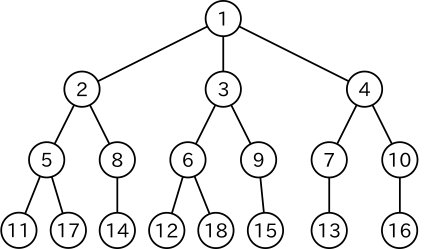
\includegraphics[width=.45\linewidth]
                    {initial-spanning-tree-18-example.pdf}
  }
  \caption{全域木初期グラフの例}
  \label{fig:initial-spanning-tree-example}
\end{figure}

定義\ref{def:stree-initial-graph}の初期グラフから探索することの
妥当性は証明されていない.次はその妥当性に関する予想である.
\begin{conjecture}\rm
  \label{conj:spanning-tree}
  一般化ムーアグラフ$M(n,k)$に,定義\ref{def:stree-initial-graph}
  で定義された全域木が存在する.
\end{conjecture}
また,条件を緩めて次も予想できる.
\begin{conjecture}\rm
  \label{conj:spanning-tree-2}
  一般化ムーアグラフ$M(n,k)$の全域木に,次の条件を満たす全域木が存在する.\par
  ある頂点$v$との距離が$Q$である頂点の集合$V=\{w\,|\,d(v,w)=Q\}$に
  ついて,次が成り立つ.
  \[ \max\{d(w)\,|\,w\in V\}-\min\{d(w)\,|\,w\in V\}\leq 1 \]
  つまり,次数の差がたかだか$1$である.
\end{conjecture}

初期グラフの変更を第\ref{chap:basic-algorithm}章で提案した方法に適応するには,
アルゴリズム\ref{algo:basic-algorithm}の2行目の$G_I$を新たに定義した
初期グラフに変更する.

\section{枝刈りによる探索空間の削減}
\label{sect:reduce-by-prune}
枝刈りによって探索空間を削減する.
本研究では,直径の下界を計算し,定理\ref{thm:gmg-geometric-property}
の条件(\ref{gmg-geom-b})を満足するか判断することで実現する.
直径の下界を計算する方法を与えるため,次のグラフを定義する.
\begin{definition}\rm
  探索途中の状態$(G,i)$に対するオペレータの適応を行う前とする.
  この状態について,グラフ$G$に候補辺番号$i$と$i$以降のすべての辺
  を追加したグラフを\textbf{最大グラフ}と定義する.
  このとき,最大グラフのもとになったグラフ$G$を\textbf{最小グラフ}と呼ぶ.
\end{definition}
\begin{example}\rm
  図\ref{fig:min-max-graph}に最小グラフと最大グラフの例を示す.
  図\ref{fig:min-graph-example}の破線部分はオペレータ適応の判定が行われていない候補辺を表す.
  最大グラフは,最小グラフのオペレータ適応未決定の辺をすべて追加したグラフと
  なっている.
\end{example}
\begin{figure}
  \centering
  \subfloat[最小グラフ(破線部分は未適応の候補辺)]{
    \includegraphics[width=.4\linewidth]
                    {min-graph-example.pdf}
    \label{fig:min-graph-example}
  }\hfill
  \subfloat[最大グラフ]{
    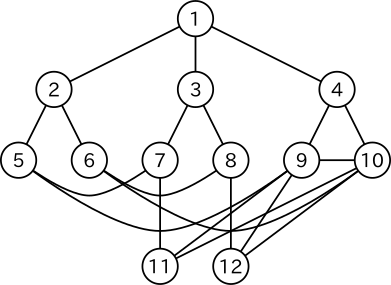
\includegraphics[width=.4\linewidth]
                    {max-graph-example.pdf}
    \label{fig:max-graph-example}
  }
  \caption{最小グラフと最大グラフの例}
  \label{fig:min-max-graph}
\end{figure}
直径の下界は,最大グラフの直径を計算すればよい.もし直径の下界が
定理\ref{thm:gmg-geometric-property}の条件(\ref{gmg-geom-b})を
満たさない場合,それ以降どのように辺を追加しても条件を満たさないので,
その場で探索を打ちきることができる.
この事実を応用して,一般化ムーアグラフの探索に直径の条件を考慮した
枝刈りをの方法を与える.探索で用いる状態は,最小グラフと最大グラフと候補辺の番号の
三つ組である.

次に,追加オペレータと無追加オペレータを新たに定めた状態に適応する.
追加オペレータは,最小グラフ$G_{\min}$と最大グラフ$G_{\max}$と候補辺番号$i$に
対して,最小グラフ$G'_{\min}=G_{\min}+e_i$と最大グラフ$G'_{\max}=G_{\max}$と
次の候補辺番号$i+1$を返す.また,無追加オペレータは,最小グラフ$G_{\min}$と
最大グラフ$G_{\max}$と候補辺番号$i$に対して,最小グラフ$G'_{\min}=G_{\min}$と
最大グラフ$G'_{\max}=G_{\max}-e_i$と次の候補辺番号$i+1$を返す.
さらに,系\ref{coll:basic-noadd-operator}で示した無追加オペレータの適応条件は
次のようになる.
\begin{corollary-without-proof}
  \label{coll:minmax-noadd-operator}
  \rm
  無追加オペレータについて,与えられた最小グラフを$G_{\min}$,最大グラフを
  $G_{\max}$,候補辺番号を$i$,対象の辺を$e_i=\{v,w\}$とし,
  適応後の最小グラフを$G'_{\min}$,最大グラフを$G'_{\max}$とする.
  $i$以降の辺の選び方次第で$G_{\min}'$が一般化ムーアグラフとなる見込み
  があることとは,次の二条件の両方を満たすことである.
  \begin{enumerate}
  \item 次数条件$\cdots$ $\text{Exit}(x)=i$なる$x\in e_i$について,
    $d_{G'_{\min}}(x)=k$.
  \item 直径条件$\cdots$ $G'_{\max}$の直径が定理\ref{thm:gmg-geometric-property}で
    示された直径以下である.
  \end{enumerate}
\end{corollary-without-proof}

本節で提案した枝刈りを第\ref{chap:basic-algorithm}章に示した方法に適応するには,
アルゴリズム\ref{algo:basic-algorithm}を次のように変更する.
\begin{itemize}
\item 4行目\ :\ $Stack\gets((G_I,G_I+\{e_i\}^M_{i\in\mathbb{N}},1))$
\item 6行目\ :\ $G,G_{\max},i\gets pop(Stack)$
\item 11行目\ :\ $operator$が$(G,G_{\max},i)$に適応できる
\item 12行目\ :\ $push(Stack,operator(G,G_{\max},i))$
\end{itemize}
さらに,各オペレータを本節で定義したものに変更する.



\chapter{実験}
\label{sect:experiment}
第\ref{chap:reduction}章で定義した初期グラフおよび枝刈りの有効性を検証する.
本章では,検証のための実験方法を示した後,結果を与えて考察を行う.

\section{実験方法}
検証のための実験方法を説明する.
実験で比較する方法は次の四種である.
\begin{enumerate}
\item 基本アルゴリズム(基本) :\ アルゴリズム\ref{algo:basic-algorithm}を
  そのまま用いる方法
\item 閉路初期グラフ(閉路) :\ アルゴリズム\ref{algo:basic-algorithm}の
  初期グラフに閉路初期グラフ(定義\ref{def:cycle-initial-graph})を用いる方法
\item 全域木初期グラフ(全域木) :\ アルゴリズム\ref{algo:basic-algorithm}の
  初期グラフに全域木初期グラフ(定義\ref{def:stree-initial-graph})を用いる方法
\item 枝刈り :\ \ref{sect:reduce-by-prune}節で提案した枝刈りを用いる方法
\end{enumerate}
実験で調べる一般化ムーアグラフの頂点数$n$と次数$k$は次のとおりである.
\begin{equation*}
  \begin{aligned}
    n=\begin{cases}
      4,6,8,10,12,14,16,18 & (k=3) \\
      5,6,7,8,9,10,11,12 & (k=4)
    \end{cases}
  \end{aligned}
\end{equation*}
評価指標には,探索開始から最初の一般化ムーアグラフを発見するまでに要する
探索時間と展開状態数を用いる.
探索時間については,それぞれの方法,頂点数,次数で10回測定してその平均を求める.
最後に本実験での実行環境を表\ref{tab:env-lab}に示す.
\begin{table}
  \caption{実行環境}
  \label{tab:env-lab}
  \centering
  \begin{tabular}{ll}
    \hline
    プロセッサ & Intel® Core™ i5-4670 CPU @ 3.40GHz × 4 \\ \hline
    メインメモリ & 5.8GiB \\ \hline
    ゲストOS & Ubuntu 16.04.3 LTS 64 ビット \\ \hline
    仮想化 & Oracle VirtualBox バージョン 5.1.18 r1140024 \\ \hline
    ホストOS & Windows 8.1 64 ビット \\ \hline
    コンパイラ & gcc 5.4.0 \\ \hline
    グラフライブラリ & igraph 0.7.1-2.1 \\ \hline
    最適化フラグ & -Ofast \\ \hline
  \end{tabular}
\end{table}

\section{結果}
探索開始から最初の一般化ムーアグラフの発見までに要した探索時間を
図\ref{fig:time}に示す.探索開始から最初の一般化ムーアグラフの発見までの
状態展開数を図\ref{fig:state}に示す.
まず,初期グラフの変更の効果について考察する.
図\ref{fig:time}と図\ref{fig:state}より,
全域木から探索を開始すれば最速かつ最も展開状態数が少ないことが分かる.
閉路初期グラフ導入後の展開状態数について,頂点数12,次数3の組合せで基本より
多くの状態を展開している.これは,候補辺列が適切な順番でなく,正則グラフであることの判定が
多くの辺が追加された後で行われていることが原因と考えられる.

次に,枝刈りの導入の効果について考察する.
図\ref{fig:state}より,枝刈りによって展開状態数が減少し,高効率化に
成功している.しかし,図\ref{fig:time}より,比較的小さい頂点数に対して,
枝刈りの導入によって探索時間が増加するような頂点数と次数の組合せがある.
必要なグラフが2個になり,より多くのグラフデータの生成と破棄が発生することで,
枝刈りによる高効率化が無効になることが原因と考えられる.
例えば,図\subref*{fig:state-d3}において頂点数14の展開状態数は少なくなっているが,
図\subref*{fig:time-d3}の頂点数14の平均探索時間は長くなっている.

\begin{figure}
  \centering
  \noindent\makebox[\textwidth]{
    \includegraphics{time-lpad.pdf}
    \includegraphics{time-ylab.pdf}
    \includegraphics{time-d3-yaxis.pdf}\hspace{-3mm}
    \subfloat[$k=3$]{
      \includegraphics{time-d3.pdf}
      \label{fig:time-d3}
    }\hspace{5mm}
    \includegraphics{time-d4-yaxis.pdf}\hspace{-3mm}
    \subfloat[$k=4$]{
      \includegraphics{time-d4.pdf}
      \label{fig:time-d4}
    }
    \includegraphics{time-legend.pdf}
  }
  \caption{最初の一般化ムーアグラフの発見までの時間}
  \label{fig:time}
\end{figure}

\begin{figure}
  \centering
  \noindent\makebox[\textwidth]{
    \includegraphics{state-lpad.pdf}
    \includegraphics{state-ylab.pdf}
    \includegraphics{state-d3-yaxis.pdf}\hspace{-3mm}
    \subfloat[$k=3$]{
      \includegraphics{state-d3.pdf}
      \label{fig:state-d3}
    }\hspace{5mm}
    \includegraphics{state-d4-yaxis.pdf}\hspace{-3mm}
    \subfloat[$k=4$]{
      \includegraphics{state-d4.pdf}
      \label{fig:state-d4}
    }
    \includegraphics{state-legend.pdf}
  }
  \caption{最初の一般化ムーアグラフの発見までの展開状態数}
  \label{fig:state}
\end{figure}



\chapter{結論}
本論文では,全探索法を基にした一般化ムーアグラフの探索の高速化および高効率化に
ついて述べた.まず,一般化ムーアグラフを定義して,その性質を示し証明を与えた.
次に,この性質を利用して,一般化ムーアグラフを探索するアルゴリズムを定めた.
最後に,探索空間の削減による高効率化の方法を与え,その効果を実験によって示した.

本論文では,高効率化の方法として,探索の初期状態を変更することと
枝刈りの二つを提案した.
探索の初期状態の変更とは,初期状態のグラフに予めいくつかの辺を追加した状態を
新たな初期状態とすることである.本論文では,辺を二本追加して閉路を含むようにした
グラフと,全域木の二種類を提案した.実験の結果から,一般的な場合では全域木から
探索を始める場合が最も効率が良いことが分かった.また,閉路を含むグラフは
ある頂点数と次数の組合せにおいて,効率が悪くなることが示された.
また,枝刈りの方法として,探索途中のグラフの直径の下界を用いる方法を提案した.
枝刈りによって探索空間が削減され高効率化は達成されたが,
頂点数および次数が小さい場合に探索に時間がかかることが結果から示された.

今後の課題は,提案した方法を用いて一般化ムーアグラフの存在を調べることや,
提案した初期状態から探索を開始することの妥当性の証明,
および,一般化ムーアグラフが存在しない時の,平均頂点間距離最小の正則グラフの
研究である.


\acknowledgment{
本論文は筆者が岡山大学工学部情報系学科に在籍中の研究結果をまとめたものである.
本研究を行うにあたり,ご指導を頂いた岡山大学大学院自然科学研究科産業創成工学専攻
高橋規一教授に深謝の意を表する.
また,情報数理工学研究室の皆様には,日常の議論を通して多くの知識や示唆を頂いた.
ここに謝意を表する.
}

\bibliography{../res/MyCollection}

\appendix

\chapter{一般化ムーアグラフのリスト}
\label{chap:list-of-gmg}
付録\ref{chap-experimental-program}で説明した\verb|exp-miner.out|を
用いて,与えられた頂点数と次数の組の一般化ムーアグラフが存在するかを
求めた.その結果を図\ref{fig:gmg-existence}に示す.
ただし,予想\ref{conj:spanning-tree}の結果次第で,存在しない組が無効になる
可能性があることに注意する.ちなみに,一般化ムーアグラフの実体は,次の
URLにて公開している.

\url{github.com/y-satotani/gmg-finder/tree/master/docs/res/graph}

\begin{figure}[htbp]
  \centering
  \captionsetup{justification=centering}
  \includegraphics{gmg-existence-v.pdf}
  \caption{頂点数と次数の一般化ムーアグラフの存在\\
    空白部分は,正則グラフが存在しない組合せもしくは,
    まだ終了していない組合せを表す.}
  \label{fig:gmg-existence}
\end{figure}


\end{document}
